% Requires: \usepackage{graphicx,tikz}
% Image paths are relative to this .tex file's location.
% Generated by: smixae latex figures  (experiment: gemma_2_9b_l20)

\begin{figure*}[t]
\centering
\noindent\makebox[\linewidth][c]{%
\begin{minipage}[t]{\linewidth}%
\vspace{0pt}\centering%
\begin{minipage}[c][4.0cm][c]{0.3267\linewidth}%
\centering%
\begin{tikzpicture}[baseline=(img.base)]
  \node[inner sep=0pt] (img) {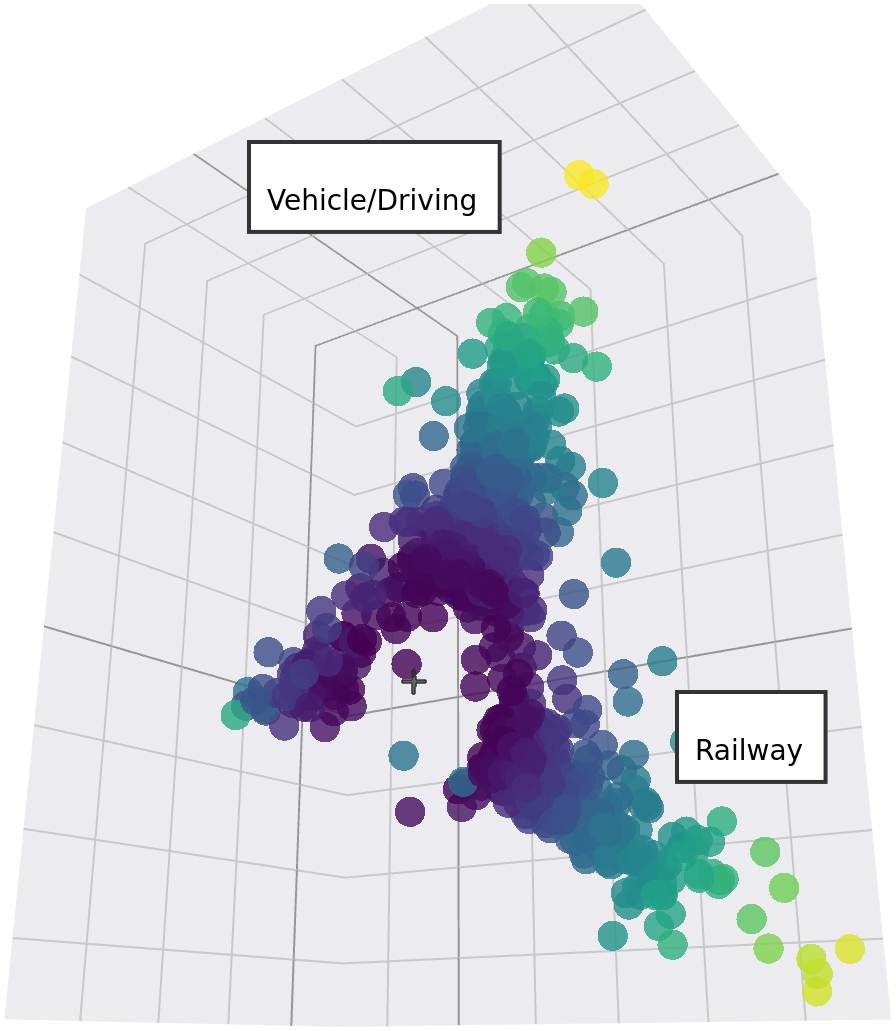
\includegraphics[width=\linewidth,height=4.0cm,keepaspectratio]{paper/camera_ready/gemma_2_9b_l20__continuity__E1360__random__cont__0.5937__scatter.png}};
  \node[anchor=north west, inner sep=2pt, overlay] at (img.north west) {\small\textbf{(a)}};
\end{tikzpicture}%
\end{minipage}%
\begin{minipage}[c][4.0cm][c]{0.3267\linewidth}%
\centering%
\begin{tikzpicture}[baseline=(img.base)]
  \node[inner sep=0pt] (img) {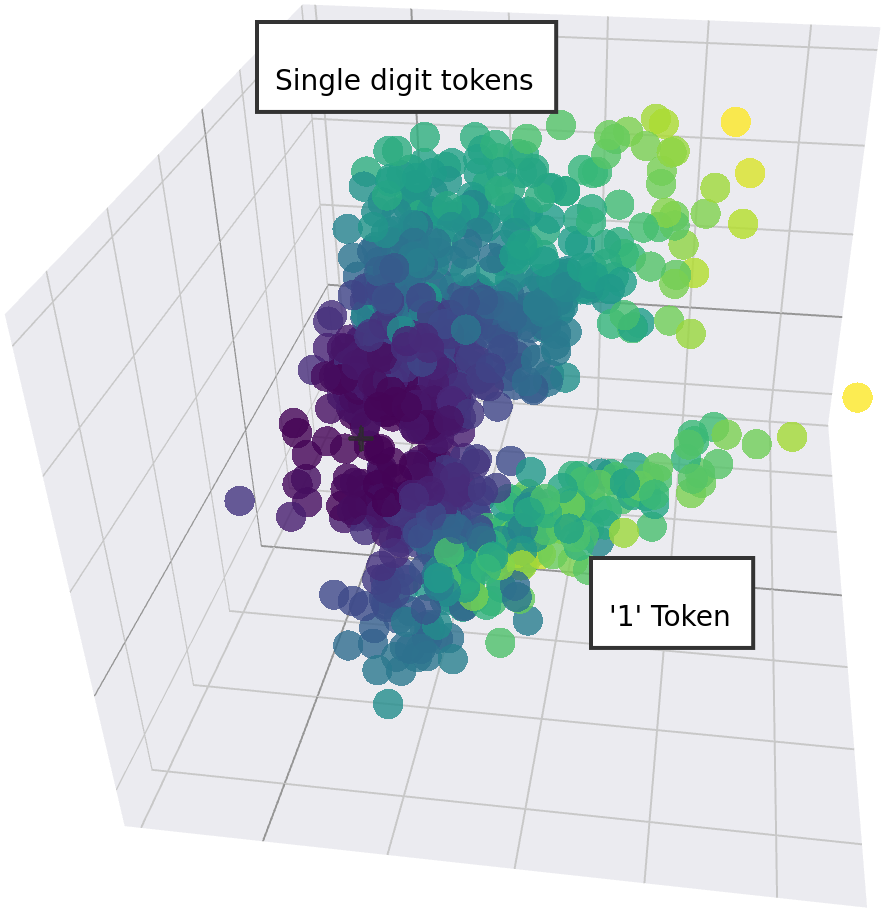
\includegraphics[width=\linewidth,height=4.0cm,keepaspectratio]{paper/camera_ready/gemma_2_9b_l20__continuity__E1567__random__cont__0.4942__scatter.png}};
  \node[anchor=north west, inner sep=2pt, overlay] at (img.north west) {\small\textbf{(b)}};
\end{tikzpicture}%
\end{minipage}%
\begin{minipage}[c][4.0cm][c]{0.3267\linewidth}%
\centering%
\begin{tikzpicture}[baseline=(img.base)]
  \node[inner sep=0pt] (img) {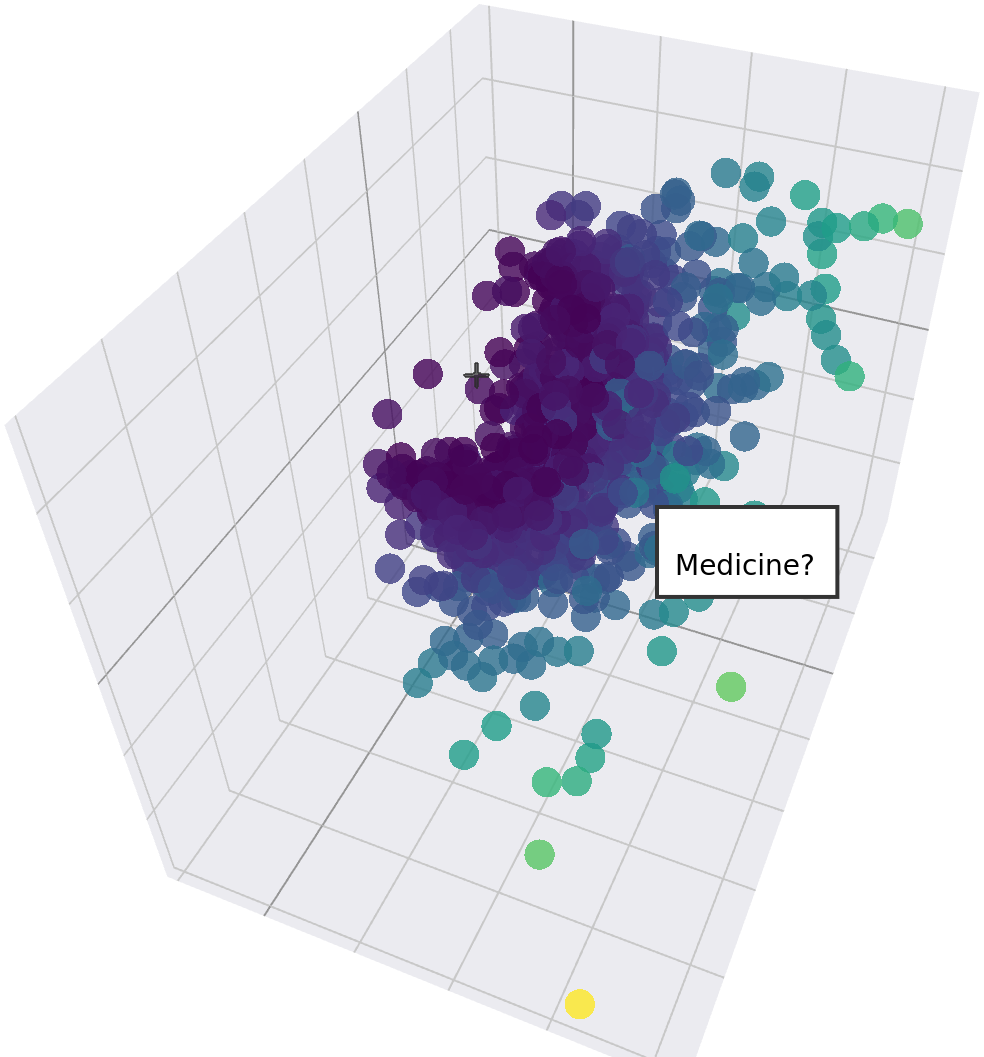
\includegraphics[width=\linewidth,height=4.0cm,keepaspectratio]{paper/camera_ready/gemma_2_9b_l20__continuity__E1578__random__cont__0.6170__scatter.png}};
  \node[anchor=north west, inner sep=2pt, overlay] at (img.north west) {\small\textbf{(c)}};
\end{tikzpicture}%
\end{minipage}%
\par\vspace{3pt}%
\begin{minipage}[c][4.0cm][c]{0.3267\linewidth}%
\centering%
\begin{tikzpicture}[baseline=(img.base)]
  \node[inner sep=0pt] (img) {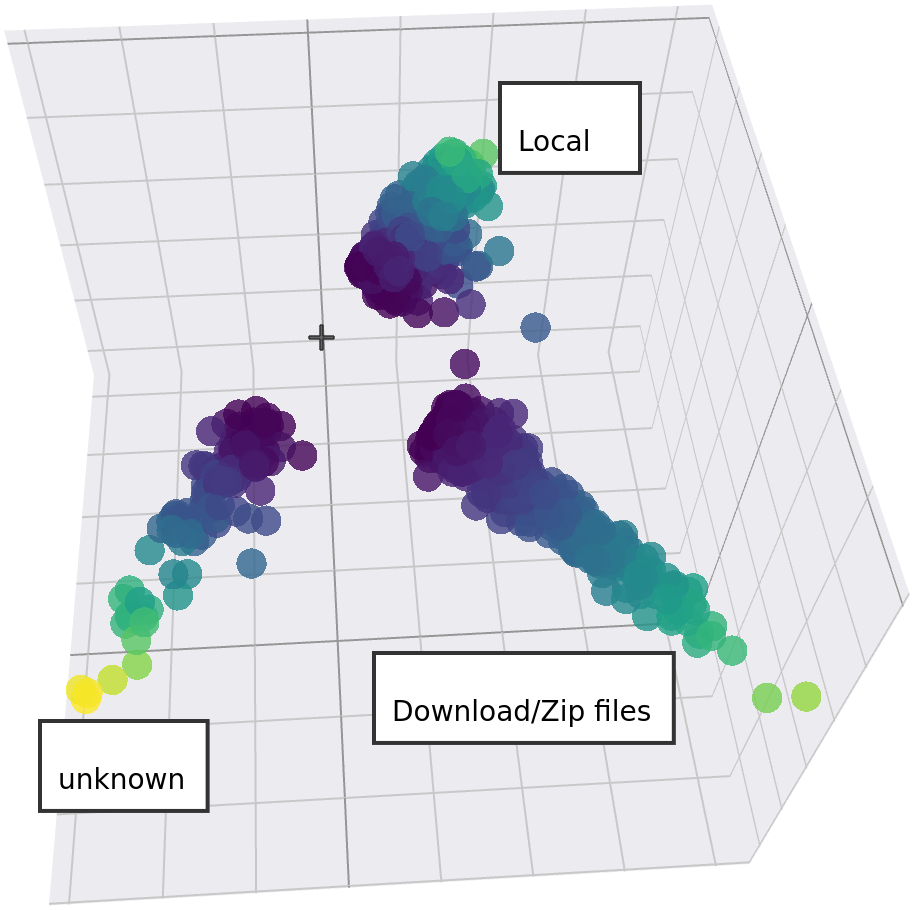
\includegraphics[width=\linewidth,height=4.0cm,keepaspectratio]{paper/camera_ready/gemma_2_9b_l20__continuity__E217__random__cont__0.5702__scatter.png}};
  \node[anchor=north west, inner sep=2pt, overlay] at (img.north west) {\small\textbf{(d)}};
\end{tikzpicture}%
\end{minipage}%
\begin{minipage}[c][4.0cm][c]{0.3267\linewidth}%
\centering%
\begin{tikzpicture}[baseline=(img.base)]
  \node[inner sep=0pt] (img) {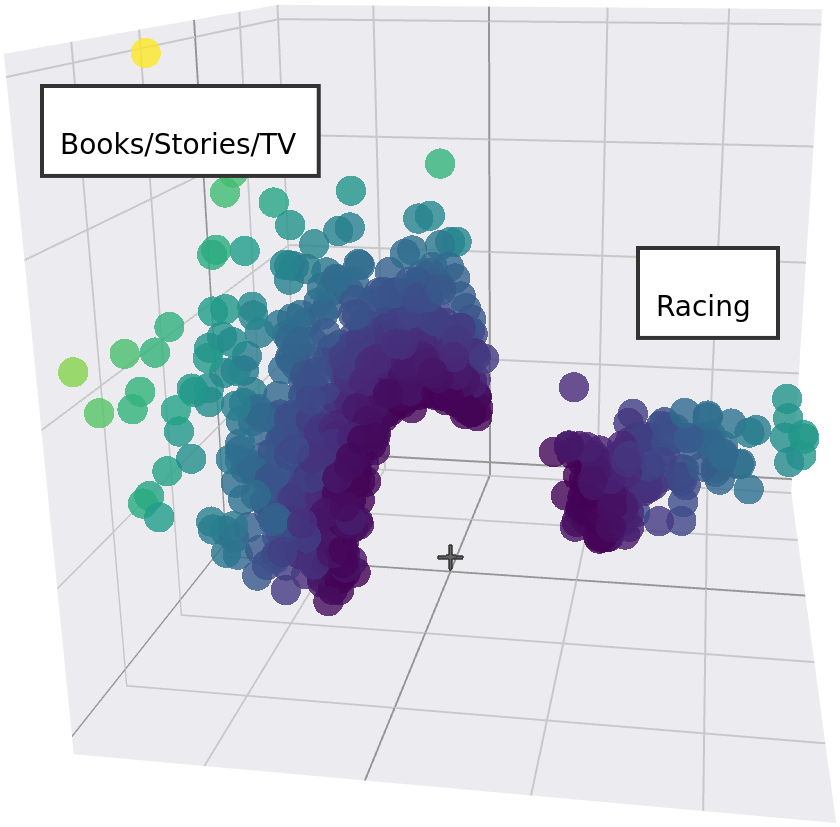
\includegraphics[width=\linewidth,height=4.0cm,keepaspectratio]{paper/camera_ready/gemma_2_9b_l20__continuity__E236__random__cont__0.6252__scatter.png}};
  \node[anchor=north west, inner sep=2pt, overlay] at (img.north west) {\small\textbf{(e)}};
\end{tikzpicture}%
\end{minipage}%
\begin{minipage}[c][4.0cm][c]{0.3267\linewidth}%
\centering%
\begin{tikzpicture}[baseline=(img.base)]
  \node[inner sep=0pt] (img) {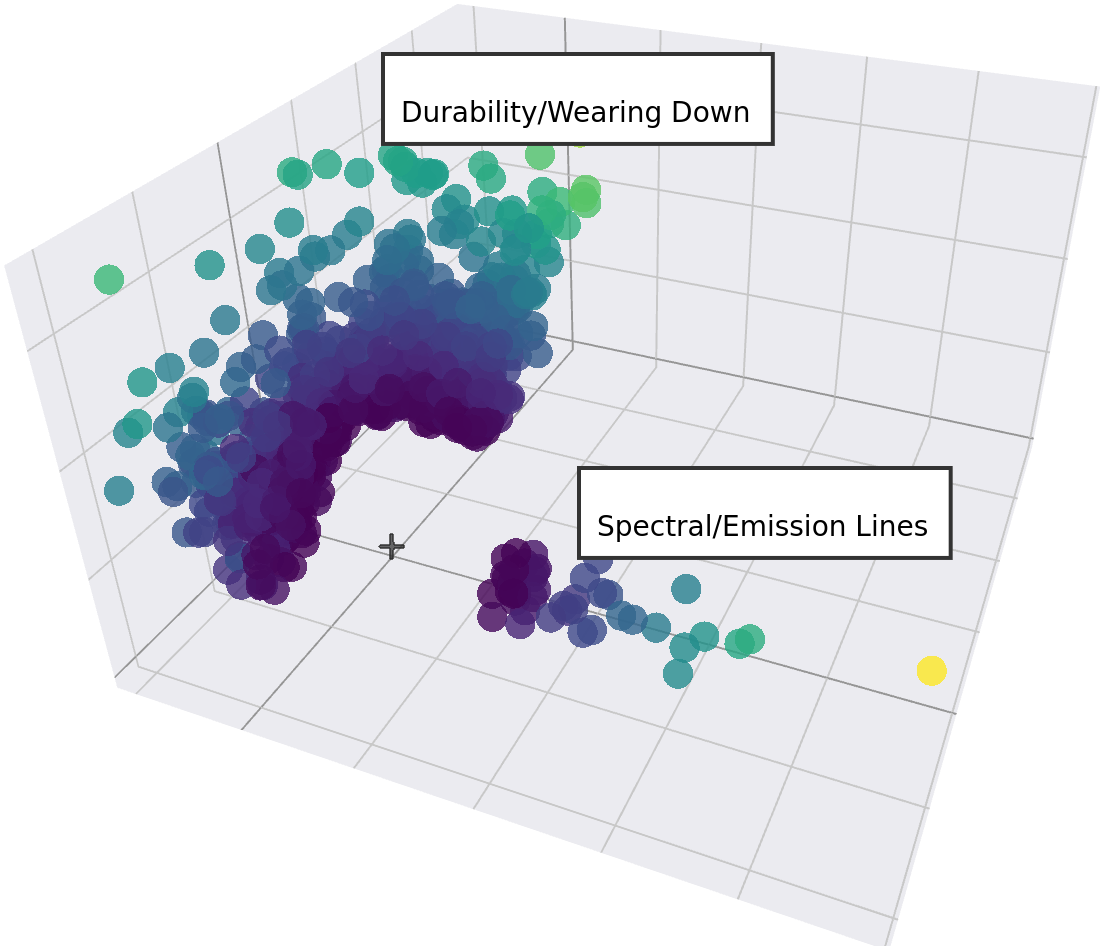
\includegraphics[width=\linewidth,height=4.0cm,keepaspectratio]{paper/camera_ready/gemma_2_9b_l20__continuity__E296__random__cont__0.6026__scatter.png}};
  \node[anchor=north west, inner sep=2pt, overlay] at (img.north west) {\small\textbf{(f)}};
\end{tikzpicture}%
\end{minipage}%
\par\vspace{3pt}%
\begin{minipage}[c][4.0cm][c]{0.3267\linewidth}%
\centering%
\begin{tikzpicture}[baseline=(img.base)]
  \node[inner sep=0pt] (img) {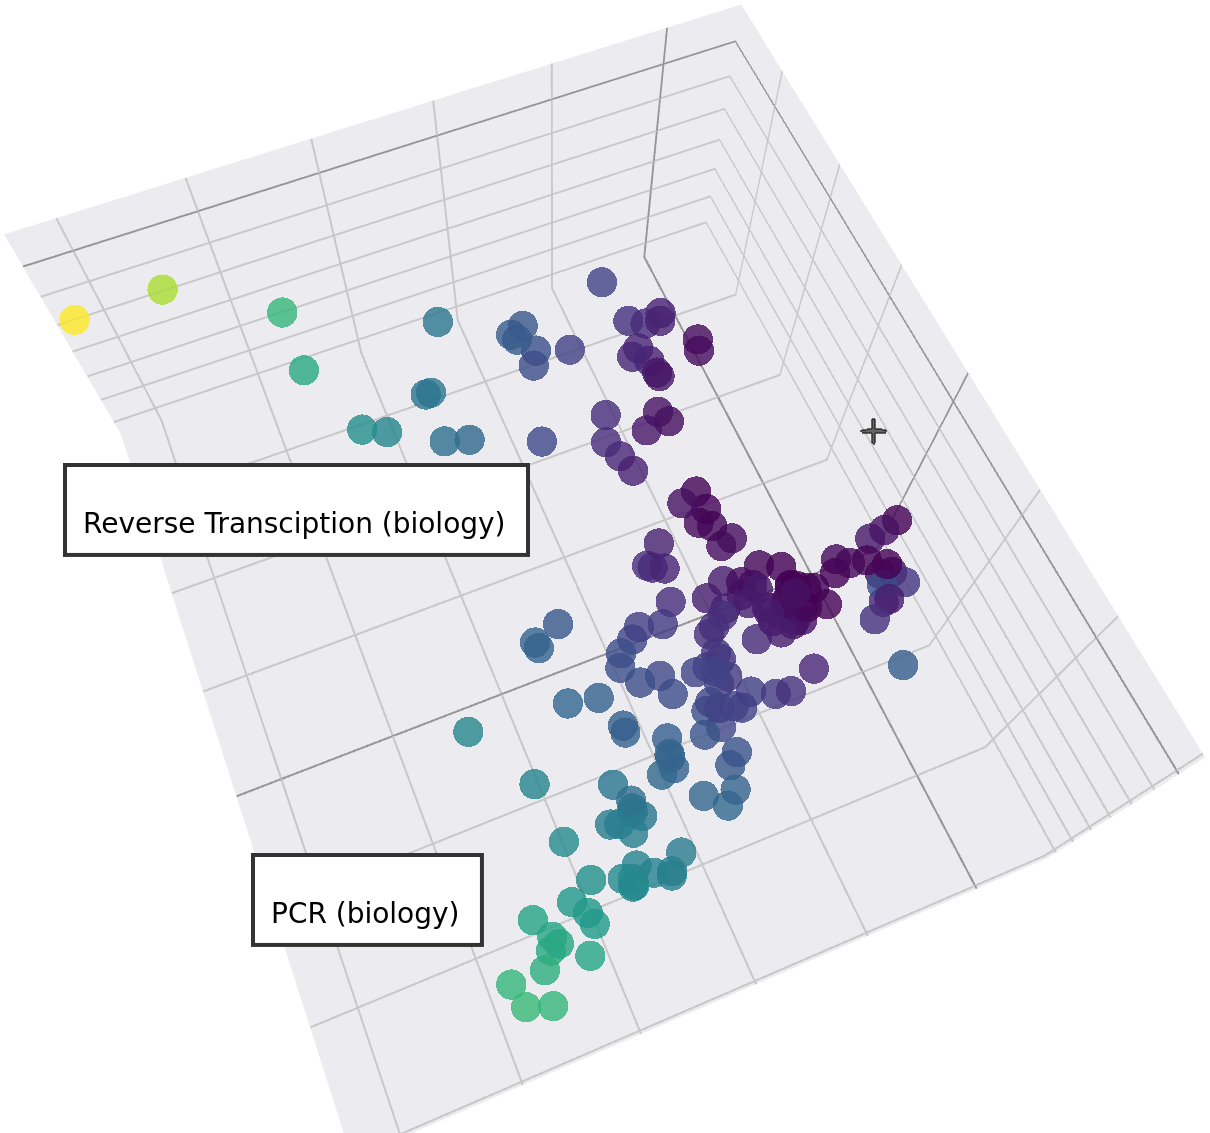
\includegraphics[width=\linewidth,height=4.0cm,keepaspectratio]{paper/camera_ready/gemma_2_9b_l20__continuity__E474__random__cont__0.6693__scatter.png}};
  \node[anchor=north west, inner sep=2pt, overlay] at (img.north west) {\small\textbf{(g)}};
\end{tikzpicture}%
\end{minipage}%
\begin{minipage}[c][4.0cm][c]{0.3267\linewidth}%
\centering%
\begin{tikzpicture}[baseline=(img.base)]
  \node[inner sep=0pt] (img) {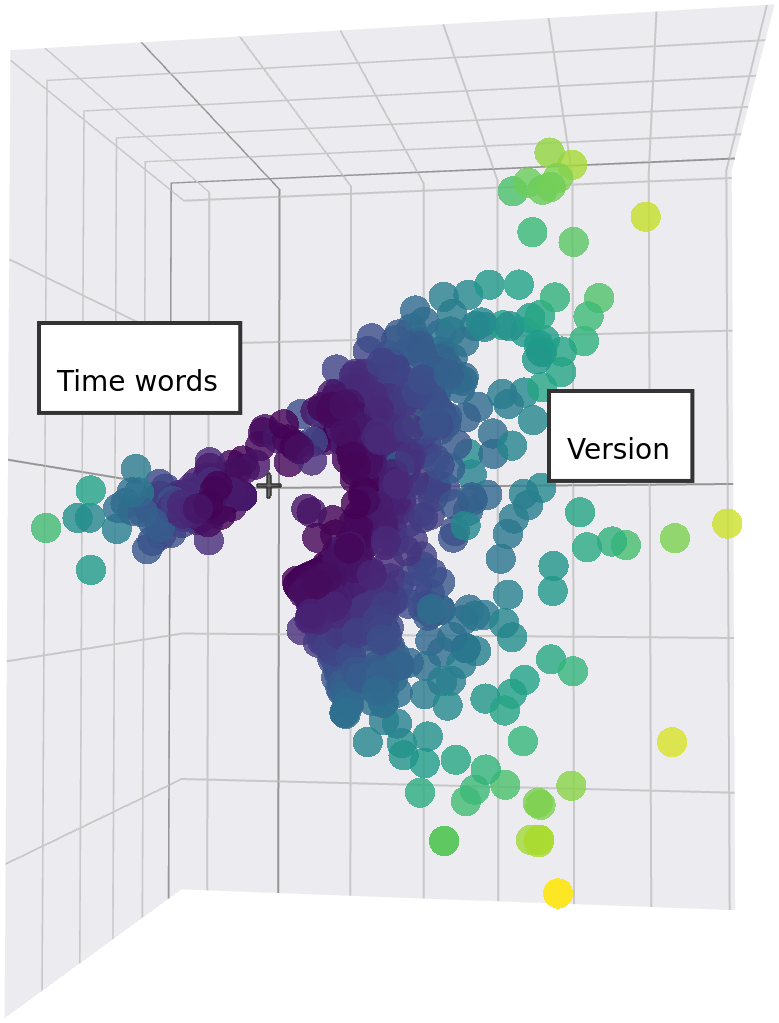
\includegraphics[width=\linewidth,height=4.0cm,keepaspectratio]{paper/camera_ready/gemma_2_9b_l20__continuity__E520__random__cont__0.5551__scatter.png}};
  \node[anchor=north west, inner sep=2pt, overlay] at (img.north west) {\small\textbf{(h)}};
\end{tikzpicture}%
\end{minipage}%
\begin{minipage}[c][4.0cm][c]{0.3267\linewidth}%
\centering%
\begin{tikzpicture}[baseline=(img.base)]
  \node[inner sep=0pt] (img) {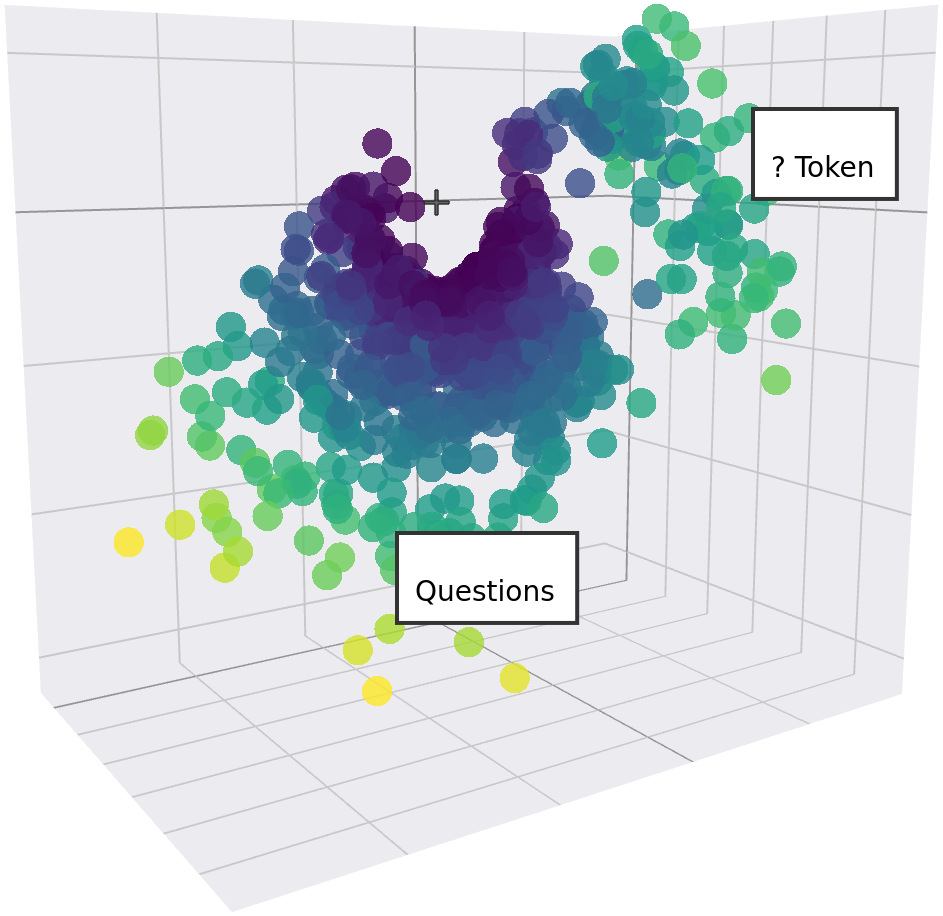
\includegraphics[width=\linewidth,height=4.0cm,keepaspectratio]{paper/camera_ready/gemma_2_9b_l20__continuity__E53__random__cont__0.6582__scatter.png}};
  \node[anchor=north west, inner sep=2pt, overlay] at (img.north west) {\small\textbf{(i)}};
\end{tikzpicture}%
\end{minipage}%
\par\vspace{3pt}%
\begin{minipage}[c][4.0cm][c]{0.3267\linewidth}%
\centering%
\begin{tikzpicture}[baseline=(img.base)]
  \node[inner sep=0pt] (img) {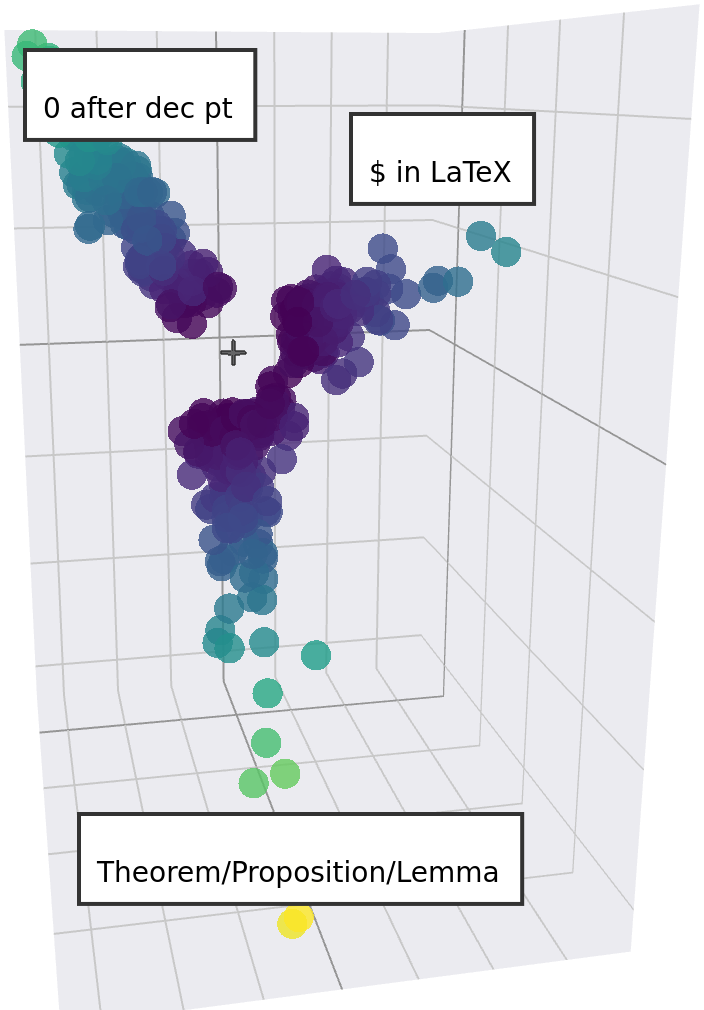
\includegraphics[width=\linewidth,height=4.0cm,keepaspectratio]{paper/camera_ready/gemma_2_9b_l20__continuity__E583__random__cont__0.6194__scatter.png}};
  \node[anchor=north west, inner sep=2pt, overlay] at (img.north west) {\small\textbf{(j)}};
\end{tikzpicture}%
\end{minipage}%
\begin{minipage}[c][4.0cm][c]{0.3267\linewidth}%
\centering%
\vspace{0pt}%
\end{minipage}%
\begin{minipage}[c][4.0cm][c]{0.3267\linewidth}%
\centering%
\vspace{0pt}%
\end{minipage}%
\par\vspace{1pt}%
{\footnotesize\textit{Random Experts (Unlabeled)}}%
\end{minipage}%
}
\caption{Gemma 2 9B, Layer 20. \textbf{Random Experts (Unlabeled)}: (a) Expert 1360, rank 1, Random Sample (Cont.\,=\,0.594). (b) Expert 1567, rank 9, Random Sample (Cont.\,=\,0.494). (c) Expert 1578, rank 4, Random Sample (Cont.\,=\,0.617). (d) Expert 217, rank 10, Random Sample (Cont.\,=\,0.570). (e) Expert 236, rank 2, Random Sample (Cont.\,=\,0.625). (f) Expert 296, rank 8, Random Sample (Cont.\,=\,0.603). (g) Expert 474, rank 7, Random Sample (Cont.\,=\,0.669). (h) Expert 520, rank 6, Random Sample (Cont.\,=\,0.555). (i) Expert 53, rank 3, Random Sample (Cont.\,=\,0.658). (j) Expert 583, rank 5, Random Sample (Cont.\,=\,0.619). Larger points denote class mean activations in the bottleneck space; smaller points are individual token activations.}
\end{figure*}
